\documentclass[a4paper, 12pt]{article}

\usepackage[utf8]{inputenc}
\usepackage[T1]{fontenc}
\usepackage[english]{babel}
\usepackage{amsmath, amssymb}
\usepackage{graphicx}
\usepackage{listings}
\usepackage[margin=0.75in, top=0.75in, bottom=0.75in]{geometry}  % Reduce all margins
\usepackage{color}
\usepackage{float}
\usepackage{hyperref}

% Define colors
\definecolor{myblue}{RGB}{0, 0, 128}
\setlength{\parindent}{0pt}



% Define code listing settings
\lstset{
    basicstyle=\ttfamily\small,
    breaklines=true,
    numbers=left,
    numberstyle=\tiny,
    frame=single,
    language=Python,
}

\title{Neural Learning - 76909 Problem Set 3}
\author{Hadar Tal}
\date{\today}

\begin{document}

\maketitle

\section*{1 The multilayer perceptron - numerical excercise}

\subsection*{1.1 Implementing the algorithm}

I have implemented the following Python functions:
\begin{lstlisting}
    predict(weights, X) ==> [predicted_labels, last_layer_activation]
    test(weights, Xtest, ytest) ==> [accuracy, mean_loss]
    backprop(weights, X, y) ==> [grads, mean_loss]
\end{lstlisting}
\bigskip
 \textcolor{myblue}{ \textbf{1.1.5} Once you finish implementing the three functions, you can train the network and see that the
classification indeed improves. Plot the batch loss over time and see if it decreases. }

I have trained the network for 6 epochs, and it reached a test accuracy of 0.932.
Here is the plot of the batch loss over time (We can see that it decreases over time): 

\begin{figure}[H]
    \centering
    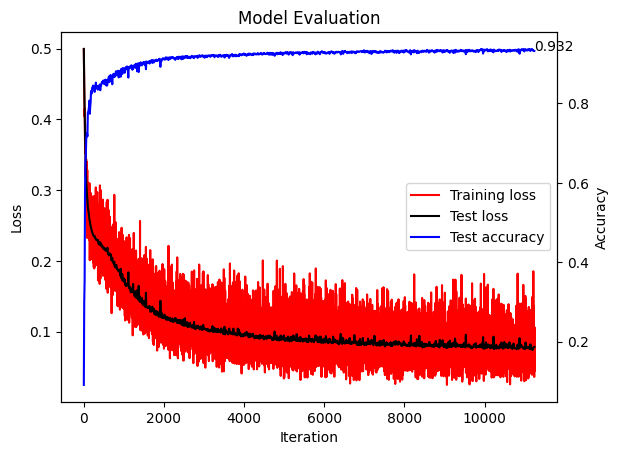
\includegraphics[width=0.6\textwidth]{../figs/1-1-5.png}   
    \caption{Learning Curve (Batch Loss over Time) and Test Loss and Accuracy} 
    \label{fig:scenario1}
\end{figure}


\subsection*{1.2 Running and Questions}

\textcolor{myblue}{
\textbf{1.2.1} Train a network with one hidden layer of 64 neurons and learning rate of $\eta$ = 0.1 for at least 4 
epochs using a batch size of 32. 
}

\begin{itemize}
    
    \item[--] \textcolor{myblue}{Display the 10 images that were misclassified with the highest loss. 
    Write down the true and predicted labels for each image.}

    \item[]
    Here are the 10 images that were misclassified with the highest loss, along with their true and predicted labels:
        
    \begin{figure}[H]
        \centering
        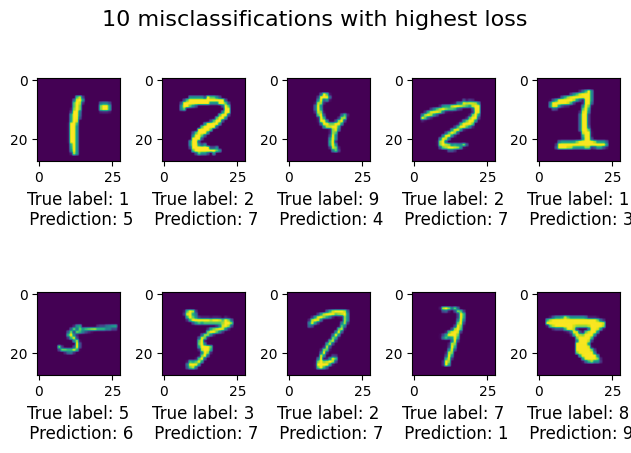
\includegraphics[width=0.6\textwidth]{../figs/1-2-1--1.png}   
        \caption{10 Images that were Misclassified with the Highest Loss} 
        \label{fig:scenario1}
    \end{figure}
    

    
    \item[--] \textcolor{myblue}{Display also 10 images that were classified correctly. }
    \item[] 
        Here are 10 images that were classified correctly:
    \begin{figure}[H]
        \centering
        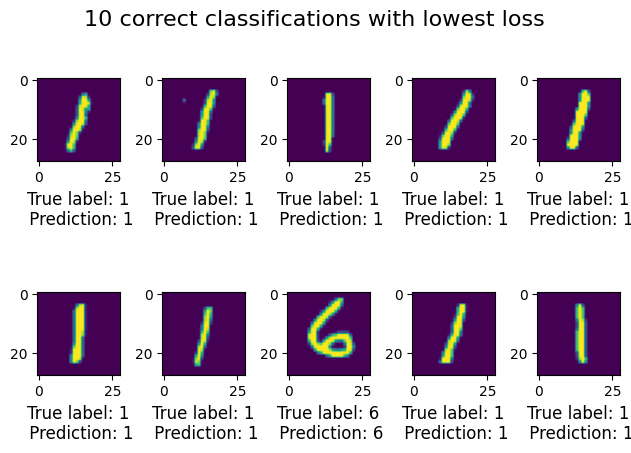
\includegraphics[width=0.6\textwidth]{../figs/1-2-1--2.png}
        \caption{10 Images that were Classified Correctly}
        \label{fig:scenario1}
    \end{figure}
    


    \item[--] \textcolor{myblue}{Do you think these images are also more (or less) ambiguous to humans?}
    \item[] 

        The images that were misclassified with the highest loss are indeed more ambiguous to humans.
        For example, the third image in the first row is a 9 that is written pretty simmilary to a 4, 
        and the second image in the second line is a 3 that is written in a very unusual way.
        The images that were classified correctly are more standard and less ambiguous.

        \smallskip
        For further analysis, I have plotted the following probability matrices:
        

        \begin{figure}[H]
            \centering
            \begin{minipage}{0.45\textwidth}
                \centering
                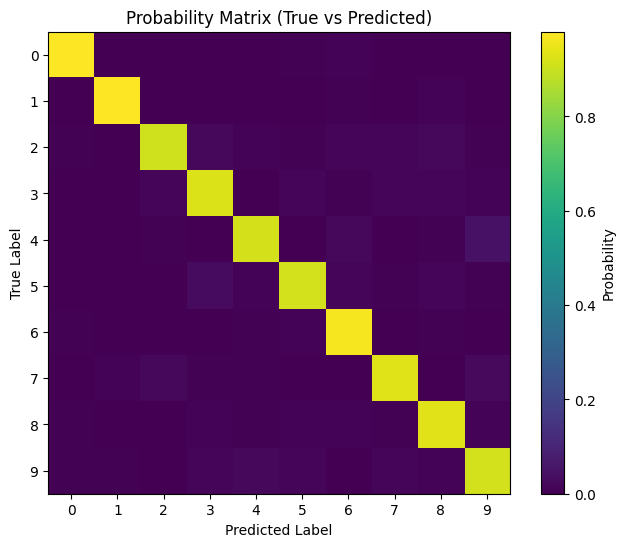
\includegraphics[width=\linewidth]{../figs/1-2-1--3.png}
                \caption{Probability Matrix (True Labels vs. Predicted Labels)}
                \label{fig:scenario1}
            \end{minipage}\hfill
            \begin{minipage}{0.45\textwidth}
                \centering
                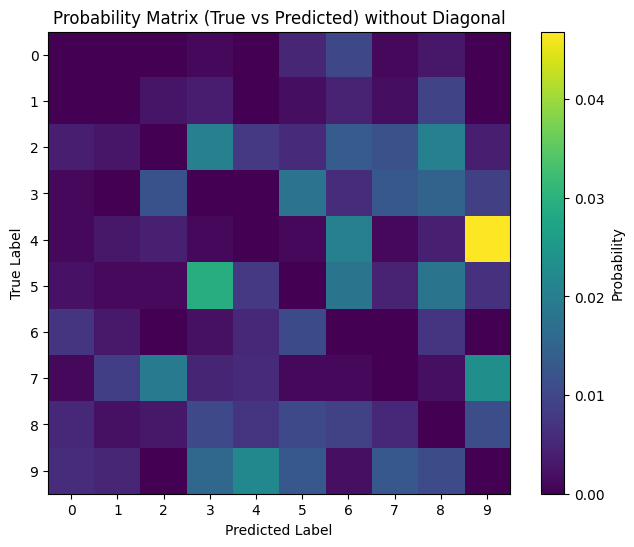
\includegraphics[width=\linewidth]{../figs/1-2-1--4.png}
                \caption{Probability Matrix (True Labels vs. Predicted Labels) without Diagonal}
                \label{fig:scenario2}
            \end{minipage}
        \end{figure}

        \smallskip
        The first matrix shows the probability of each true label to be predicted as each label.
        The second matrix is the same, but without the diagonal, to emphasize the misclassifications.
        From the second matrix, we can see that the most common misclassifications are 4 as 9 and 5 as 3.
            
        \begin{figure}[H]
            \centering
            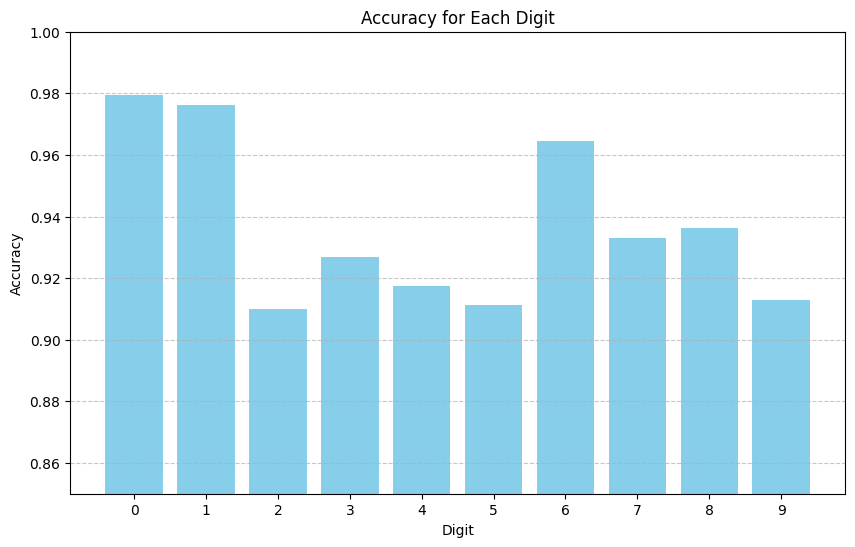
\includegraphics[width=0.8\textwidth]{../figs/1-2-1--5.png}
            \caption{Accuracy for Each Digit}
            \label{fig:scenario1}
        \end{figure}

\end{itemize}

\bigskip

\textcolor{myblue}{
    \textbf{1.2.2} Train the network with the same parameters as above but with learning rates $\eta$ = 0.01, 0.1 and
1. Plot the average training loss on the batches throughout the training. Explain the differences
between the learning curves.
}

Here are the plots of the average training loss on the batches throughout the training for the three learning rates:

\begin{figure}[H]
    \centering
    \begin{minipage}{0.45\textwidth}
        \centering
        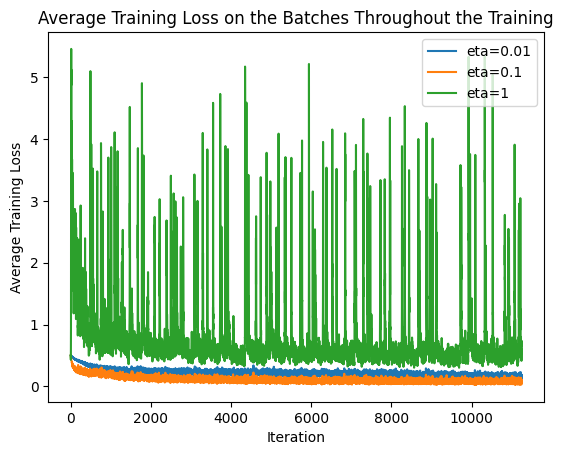
\includegraphics[width=\linewidth]{../figs/1-2-2--1.png}
        \caption{Average Training Loss on Batches throughout the Training for Different Learning Rates}
        \label{fig:scenario1}
    \end{minipage}\hfill
    \begin{minipage}{0.45\textwidth}
        \centering
        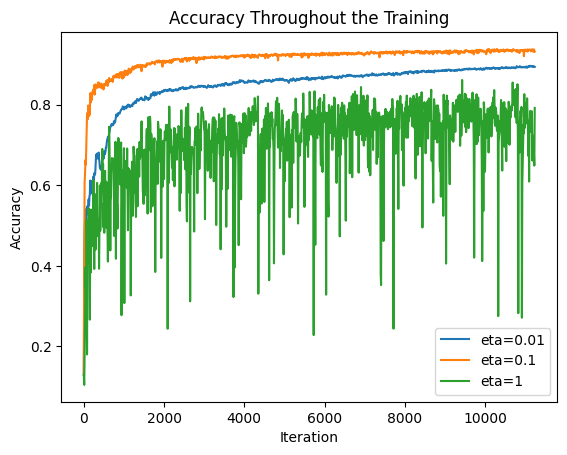
\includegraphics[width=\linewidth]{../figs/1-2-2--2.png}
        \caption{Accuracy throughout the Training for Different Learning Rates}
        \label{fig:scenario2}
    \end{minipage}
\end{figure}


We can see that the learning rate of 0.01 is too low, and the network converges very slowly.
The learning rate of 1 is too high, and the network diverges.
The learning rate of 0.1 is the best, and the network converges quickly.


\bigskip
\textcolor{myblue}{
\textbf{1.2.3} Train vs. Test: Train a network with one hidden layer of 32 neurons on a subset of 100 random
images from the training set but uniform across lables, i.e. 10 of each digit. Use a learning
rate of $\eta$ = 0.1 and batch size of 32. Run the algorithm until the training loss seems to converge
(about 200 epochs since we have a small training set). 
}

\begin{itemize}
    \item[--] \textcolor{myblue}{Plot the training loss, test loss, and test error (i.e. 1-accuracy) throughout the training.}
    
    \item[] Bellow are the plots (the batch loss and test loss are normalized by the maximum value of the batch loss and test loss, respectively, for better visualization.)
    
    \begin{figure}[H]
        \centering
        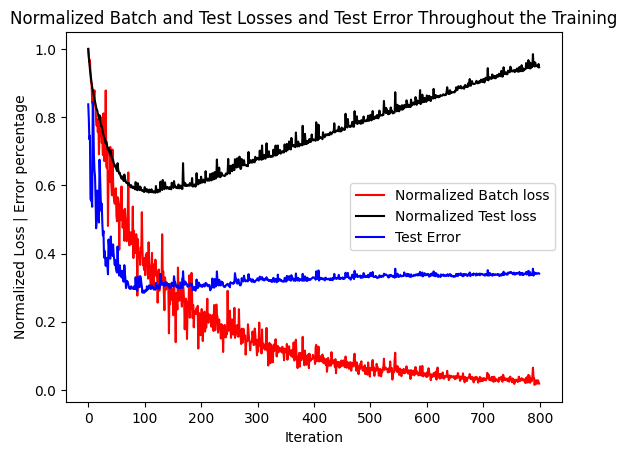
\includegraphics[width=0.8\textwidth]{../figs/1-2-3--1.png}
        \caption{Normalized Batch and Test Losses and Test Error Throughout the Training}
        \label{fig:scenario1}
    \end{figure}

    \item[(a)] \textcolor{myblue}{In your opinion, does the training sample match the true statistics of hand written digits?
    Explain.}
    \item[] 
        In my opinion, the training sample may not fully match the true statistics of handwritten digits. 
        The data shows that both batch loss and test loss initially decrease until approximately the 100th iteration,
        where we achieve a minimal error rate of approximately 29\%. 
        However, from iteration 100 to 800, while the batch loss continues to decrease, 
        both test loss and error rate increase. 
        This divergence in trends suggests potential shortcomings in the training sample's representation 
        of true handwritten digit statistics. The increasing error rate indicates the possibility of 
        overfitting to the training data. 
        In scenarios where the training sample accurately reflects the diversity of handwritten digits, 
        one would expect better generalization to unseen data, with test loss and error ideally 
        decreasing or stabilizing over training iterations. 
        owever, the observed discrepancy underscores the importance of training data diversity. 
        While our sample contains 10 images of each digit, the true distribution of handwritten 
        digits in real-world data may be more varied, potentially limiting the model's ability to generalize effectively.

    \item[(b)] \textcolor{myblue}{A common heuristic to avoid over-fitting of gradient descent methods and improve test
    performance is early stopping - stopping the algorithm before the training error converges. Based on the results, would it have made sense to do so in our case?}
    \item[] 
    Yes, based on the results indicating that both batch loss and test loss decrease until approximately the 100th 
    iteration, after which test loss and error rate start to increase while batch loss continues to decrease, 
    implementing early stopping could have been beneficial in our case. 
    By stopping the training process earlier, we could have obtained a model with 
    better generalization performance, potentially avoiding the overfitting observed in later iterations.

\end{itemize}

\bigskip
\textcolor{myblue}{
\textbf{1.2.4} Run the same network as before (32 hidden neurons) but use the whole training set this time.
Since we use many more samples, 4 epochs should be enough for convergence.  
}

\begin{itemize}
    \item[--] \textcolor{myblue}{Plot the same figure as before.}
    
    \begin{figure}[H]
        \centering
        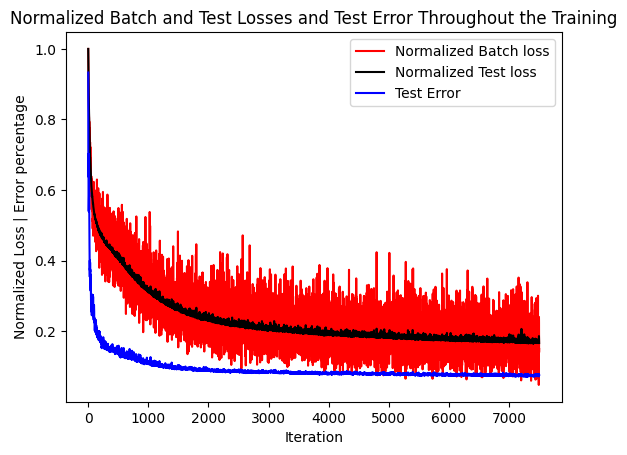
\includegraphics[width=0.8\textwidth]{../figs/1-2-4--1.png}
        \caption{Normalized Batch and Test Losses and Test Error Throughout the Training}
        \label{fig:scenario1}
    \end{figure}
    
    \item[--] \textcolor{myblue}{What is different this time? How will early stopping affect the test error now?}
    \item[] With all curves decreasing, indicating effective learning from the entire training set, 
    early stopping could potentially increase the error rate. 
    Since the decreasing curves suggest that the model is converging well and not overfitting, 
    prematurely stopping the training process might prevent the model from fully optimizing its performance. 
    Early stopping is typically employed to prevent overfitting by halting training before the model 
    memorizes the training data excessively. 
    However, if the model is already converging effectively, interrupting the training prematurely 
    could hinder its ability to further refine its understanding of the data, potentially resulting 
    in a higher test error rate than if training had continued. 
    Therefore, in this scenario, early stopping might not only fail to significantly 
    improve the test error but could also potentially lead to an increase in the error rate.

\end{itemize}

\section*{2 Gradient descent with momentum}

\textcolor{myblue}{
\textbf{2.1} {Solve this difference equation and obtain an expression for $\Delta w_{ij}^{n}$ 
as a function of $\alpha$, $\eta$ and the series of gradients
 $\left\{ \frac{\partial E_{t}}{\partial w_{ij}^{t}} \right\} $.
at all times previous to the update t = 1, \dots,  n.
    }
}

\begin{align*}
    \Delta w_{ij}^{n} &= \alpha \Delta w_{ij}^{n-1} - \eta \frac{\partial E_{n}}{\partial w_{ij}^{n}} \\
    &= \alpha \left( \alpha \Delta w_{ij}^{n-2} - \eta \frac{\partial E_{n-1}}{\partial w_{ij}^{n-1}} \right) - \eta \frac{\partial E_{n}}{\partial w_{ij}^{n}} \\
    &= \alpha^2 \Delta w_{ij}^{n-2} - \alpha \eta \frac{\partial E_{n-1}}{\partial w_{ij}^{n-1}} - \eta \frac{\partial E_{n}}{\partial w_{ij}^{n}} \\
    &= \alpha^3 \Delta w_{ij}^{n-3} - \alpha^2 \eta \frac{\partial E_{n-2}}{\partial w_{ij}^{n-2}} - \alpha \eta \frac{\partial E_{n-1}}{\partial w_{ij}^{n-1}} - \eta \frac{\partial E_{n}}{\partial w_{ij}^{n}} \\
    &= \alpha^n \Delta w_{ij}^{0} - \eta \sum_{k=0}^{n-1} \alpha^{k} \frac{\partial E_{n-k}}{\partial w_{ij}^{n-k}} \\
\end{align*}

\end{document}


% \begin{figure}[h]
%     \centering
%     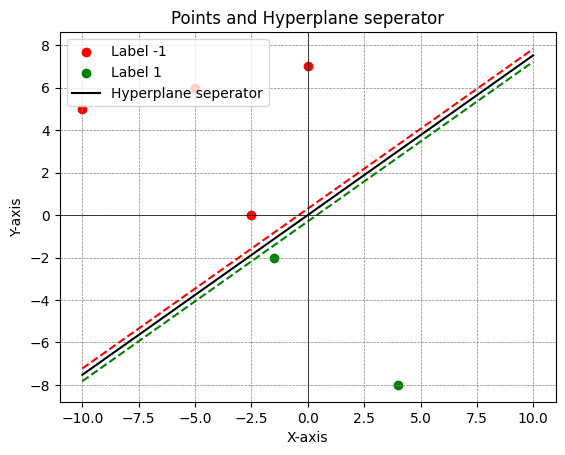
\includegraphics[width=0.6\textwidth]{./assets/nn_ex1_3_1.png}
% \end{figure}

% \subsection*{1.2 Binary Perceptron Learning Algorithm (for $P < N$)}
% The graph below illustrates the relationship between $N$ (points' dimension) and the
% number of epochs required for convergence ($P=10$ for all iterations).
% From the graph, we can infer that the number of epochs decreases as $N$ increases until some $\hat{N}$,
% where for all $n > \hat{N}$, it becomes approximately a constant number.
% As seen in class, for $P < N$, an optimal $w$ is of the form:
% \[ w^\star = \sum_{\mu = 1}^{P} (Q^{-1}y_0)_{\mu} x^{\mu} + w_{\bot }\]
% where $w_{\bot }$ is an arbitrary vector perpendicular to all examples,
% and ${Q}_{\mu \nu } \equiv  {(x^\mu)}^T x^\nu$.
% As the dimensionality increases, the volume of the space grows exponentially.
% In higher-dimensional spaces, points become more spread out, and it becomes easier to find a hyperplane that separates them.
